% !TEX TS-program = xelatex
% !TEX encoding = UTF-8 Unicode
% !Mode:: "TeX:UTF-8"

\documentclass{resume}
\usepackage{zh_CN-Adobefonts_external} % Simplified Chinese Support using external fonts (./fonts/zh_CN-Adobe/)
%\usepackage{zh_CN-Adobefonts_internal} % Simplified Chinese Support using system fonts
\usepackage{linespacing_fix} % disable extra space before next section
\usepackage{graphicx}
\usepackage{tabu}
\usepackage{multirow}

\begin{document}
\pagenumbering{gobble} % suppress displaying page number

\large{
  \begin{tabu}{ c l }
   \multirow{5}{1in}{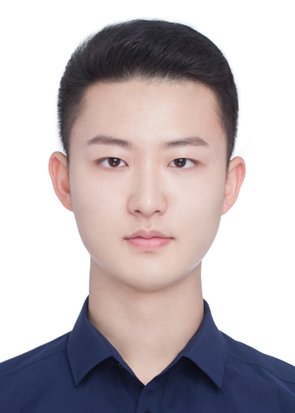
\includegraphics[width=0.88in]{avatar-1}} & \\ & \scshape \LARGE {\, 孙东旭}  \\
    & \quad \email{371211947@qq.com}  \\
    & \quad \phone{(+86) 189-7308-9012}  \\
    & \quad \github{https://github.com/sundongxu} \\
    & \quad 
\includegraphics[scale=0.02]{blog.pdf}{\ http://dongdongdong.me}
  \end{tabu} 
  \\ \\ 
  
\section{\faGraduationCap\  教育背景}
\datedsubsection{\textbf{南京大学}}{2016 - 至今}
\normalsize
\textit{在读硕士研究生} \quad 计算机科学技术系 \quad 分布式计算
\datedsubsection{\textbf{大连理工大学}}{2012 - 2016}
\normalsize
\textit{学士} \quad 国家示范性软件学院 \quad 软件工程 

\section{\faUsers\ 实习/项目经历}
\datedsubsection{\textbf{腾讯} \quad MIG \quad 应用宝 \quad 游戏产品中心}{2015.08 -- 2016.02}
\normalsize
\role{实习}{移动客户端开发}
\begin{itemize}
  \item 参与并完成福利中心Native导航改版、游戏页NPC弹窗、新版智能卡片、游戏内icon及预约弹框优化等多项需求,后经灰度、测试均已发布上线
  \item 2015年末代表MIG参与并主演公司年会(圣诞晚会)节目《白毛女》
  \item 作为主力先后代表应用宝与MIG参加BG内部及公司BG篮球联赛,分获亚军、季军
\end{itemize}

\datedsubsection{\textbf{RDMA网络中间件}}{2017.01 - 2017.06}
\normalsize
\role{C++/C}{科研项目,与组员合作开发}
提供类Socket接口的高性能网络库
\begin{itemize}
  \item 支持上层应用使用RDMA替换TCP/IP完成网络操作(消息语义、内存语义)
  \item 涉及技术:TCP/IP与RDMA协议栈、多线程并发同步、内存管理、epoll多路复用等 
  \item 在memcached、grpc等开源项目中测试通过
\end{itemize}

\datedsubsection{\textbf{个人理财APP}}{2016.03 - 2016.05}
\normalsize
\role{Android(Java)}{个人项目}
嵌入个性化推荐算法的虚拟理财平台, https://github.com/sundongxu/personal-financing
\begin{itemize}
  \item 基于安卓平台,采用material design设计原则
  \item 实现功能:卡片展现、模拟投资、明细记账、生活备忘等
  \item 涉及技术:网络请求(volley)、数据库(sqlite)、文件I/O等
\end{itemize}

\datedsubsection{\textbf{沫梦音乐网}}{2014.05 - 2014.07}
\normalsize
\role{J2EE}{兴趣项目}
\begin{itemize}
  \item 基本框架:JavaBean + Sevlet + JSP + JDBC
  \item 实现功能:歌曲上传、查找、按点击和搜索次数排行、删除等
\end{itemize}

\section{\faCogs\ 技术栈}
% increase linespacing [parsep=0.5ex]
\begin{itemize}[parsep=0.5ex]
  \item 语言: C++ == Java > Python
  \item 平台: Linux/MacOS
  \item 自评:理解面向对象思想,熟悉基本数据结构及常用算法,并熟练掌握C++及GCC、GDB及Vim等相关开发工具的使用;多次Java(Android)项目经历,并能利用Python(Numpy、Pandas、Matplotlib)进行数据分析;长期工作在Linux系统环境下,熟悉常用命令,了解基本Shell脚本编程;对网络编程及内核原理兴趣浓厚(钻研中)
\end{itemize}

\end{document}
